\documentclass[11pt,border=5pt]{standalone}
\usepackage{fontspec}
\setmainfont{cmunrm.otf}[BoldFont=cmunbx.otf,ItalicFont=cmunti.otf,BoldItalicFont=cmunbi.otf]
\usepackage{amsmath}
\usepackage{unicode-math}
\setmathfont{NewCMMath-Regular.otf}
\usepackage{tikz}
\usetikzlibrary{arrows.meta,patterns,angles,quotes}
\begin{document}
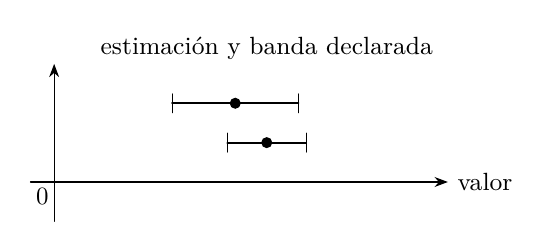
\begin{tikzpicture}[>=Stealth,font=\small,line cap=round,line join=round]
\draw[->,thin] (-0.3,0) -- (5,0) node[pos=1,right] {valor};
\draw[->,thin] (0,-0.5) -- (0,1.5);
\node at (-0.14,-0.18) {$0$};
\draw[thick] (1.4999999999999998,1) -- (3.0999999999999996,1);
\draw[] (1.4999999999999998,0.88) -- (1.4999999999999998,1.12);
\draw[] (3.0999999999999996,0.88) -- (3.0999999999999996,1.12);
\fill (2.3,1) circle (2pt);
\draw[thick] (2.2,0.5) -- (3.2,0.5);
\draw[] (2.2,0.38) -- (2.2,0.62);
\draw[] (3.2,0.38) -- (3.2,0.62);
\fill (2.7,0.5) circle (2pt);
\node at (2.7,1.7) {estimación y banda declarada};

\end{tikzpicture}
\end{document}
